\documentclass{article}

\usepackage{geometry}

\geometry{a4paper}

% \usepackage[UTF8, heading = false, scheme = plain]{ctex}%格式

% \usepackage{ctex}

%\usepackage{authblk} %添加机构 安装preprint后可用

\usepackage{graphicx} %添加图片
\usepackage{listings}
\usepackage{float}  %设置图片浮动位置的宏包
\usepackage{subfigure}  %插入多图时用子图显示的宏包
\usepackage{amsthm}
\usepackage{booktabs}       % professional-quality tables
\usepackage{amsfonts}       % blackboard math symbols
\usepackage{nicefrac}       % compact symbols for 1/2, etc.
\usepackage{microtype}      % microtypography
\usepackage{multirow}
\usepackage{caption}

% \usepackage{subcaption}
% \usepackage{fontspec} % 定制字体

\usepackage{xcolor} % 定制颜色
\definecolor{mygreen}{rgb}{0,0.6,0}
\definecolor{mygray}{rgb}{0.5,0.5,0.5}
\definecolor{mymauve}{rgb}{0.58,0,0.82}
\lstset{ %
backgroundcolor=\color{white},      % choose the background color
basicstyle=\footnotesize\ttfamily,  % size of fonts used for the code
columns=fullflexible,
tabsize=4,
breaklines=true,               % automatic line breaking only at whitespace
captionpos=b,                  % sets the caption-position to bottom
commentstyle=\color{mygreen},  % comment style
escapeinside={\%*}{*)},        % if you want to add LaTeX within your code
keywordstyle=\color{blue},     % keyword style
stringstyle=\color{mymauve}\ttfamily,  % string literal style
frame=single,
rulesepcolor=\color{red!20!green!20!blue!20},
% identifierstyle=\color{red},
language=python,
}


\usepackage{amsmath}

\renewcommand{\vec}[1]{\boldsymbol{#1}} % 生产粗体向量,而不是带箭头的向量
\renewcommand{\thesubfigure}{(\arabic{subfigure})}
\usepackage{amssymb}

\usepackage{booktabs} % excel导出的大表格

\usepackage{hyperref}

%\newtheorem{definition}{Definition} %英文
% \setCJKmainfont{hk4e_zh-cn.ttf}     % 语义和语法同fontspec
% \setCJKsansfont{hk4e_zh-cn.ttf}
% \setCJKmonofont{hk4e_zh-cn.ttf}
% \setmainfont{hk4e_zh-cn.ttf}
% \setsansfont{hk4e_zh-cn.ttf}
% \setmonofont{hk4e_zh-cn.ttf}
%\newtheorem{theorem}{Theorem}
\geometry{a4paper,scale=0.8}
% \newtheorem{definition}{定义} %中文

% \newtheorem{lemma}{引理}

% \newtheorem{theorem}{定理}

%\newenvironment{proof}{{\noindent\it 证明}\quad}{\hfill □ \square□\par}

\DeclareMathOperator{\Ima}{Im}%定义新符号

\DeclareMathOperator{\Rank}{rank}%定义求秩算子

\title{Machine Learning Personal Project}

\author{Jiang Shuyang \\ Email: \href{mailto:jiangshuyang@sjtu.edu.cn}{jiangshuyang@sjtu.edu.cn}}

%\affil{中国科学院} 
%需要把上面的\usepackage{authblk}取消注释

%date{}

\begin{document}

\maketitle

\section{Introduction}
In this project, I finish the basic task, i.e., image classification on MNIST dataset. Besieds, I also finish image generation with VAE and sentiment analysis with LSTM. I will in detail illustrate the model architectures in each task, final result on test set and corresponding visualization results.

\begin{figure}[htbp]
    \centering
    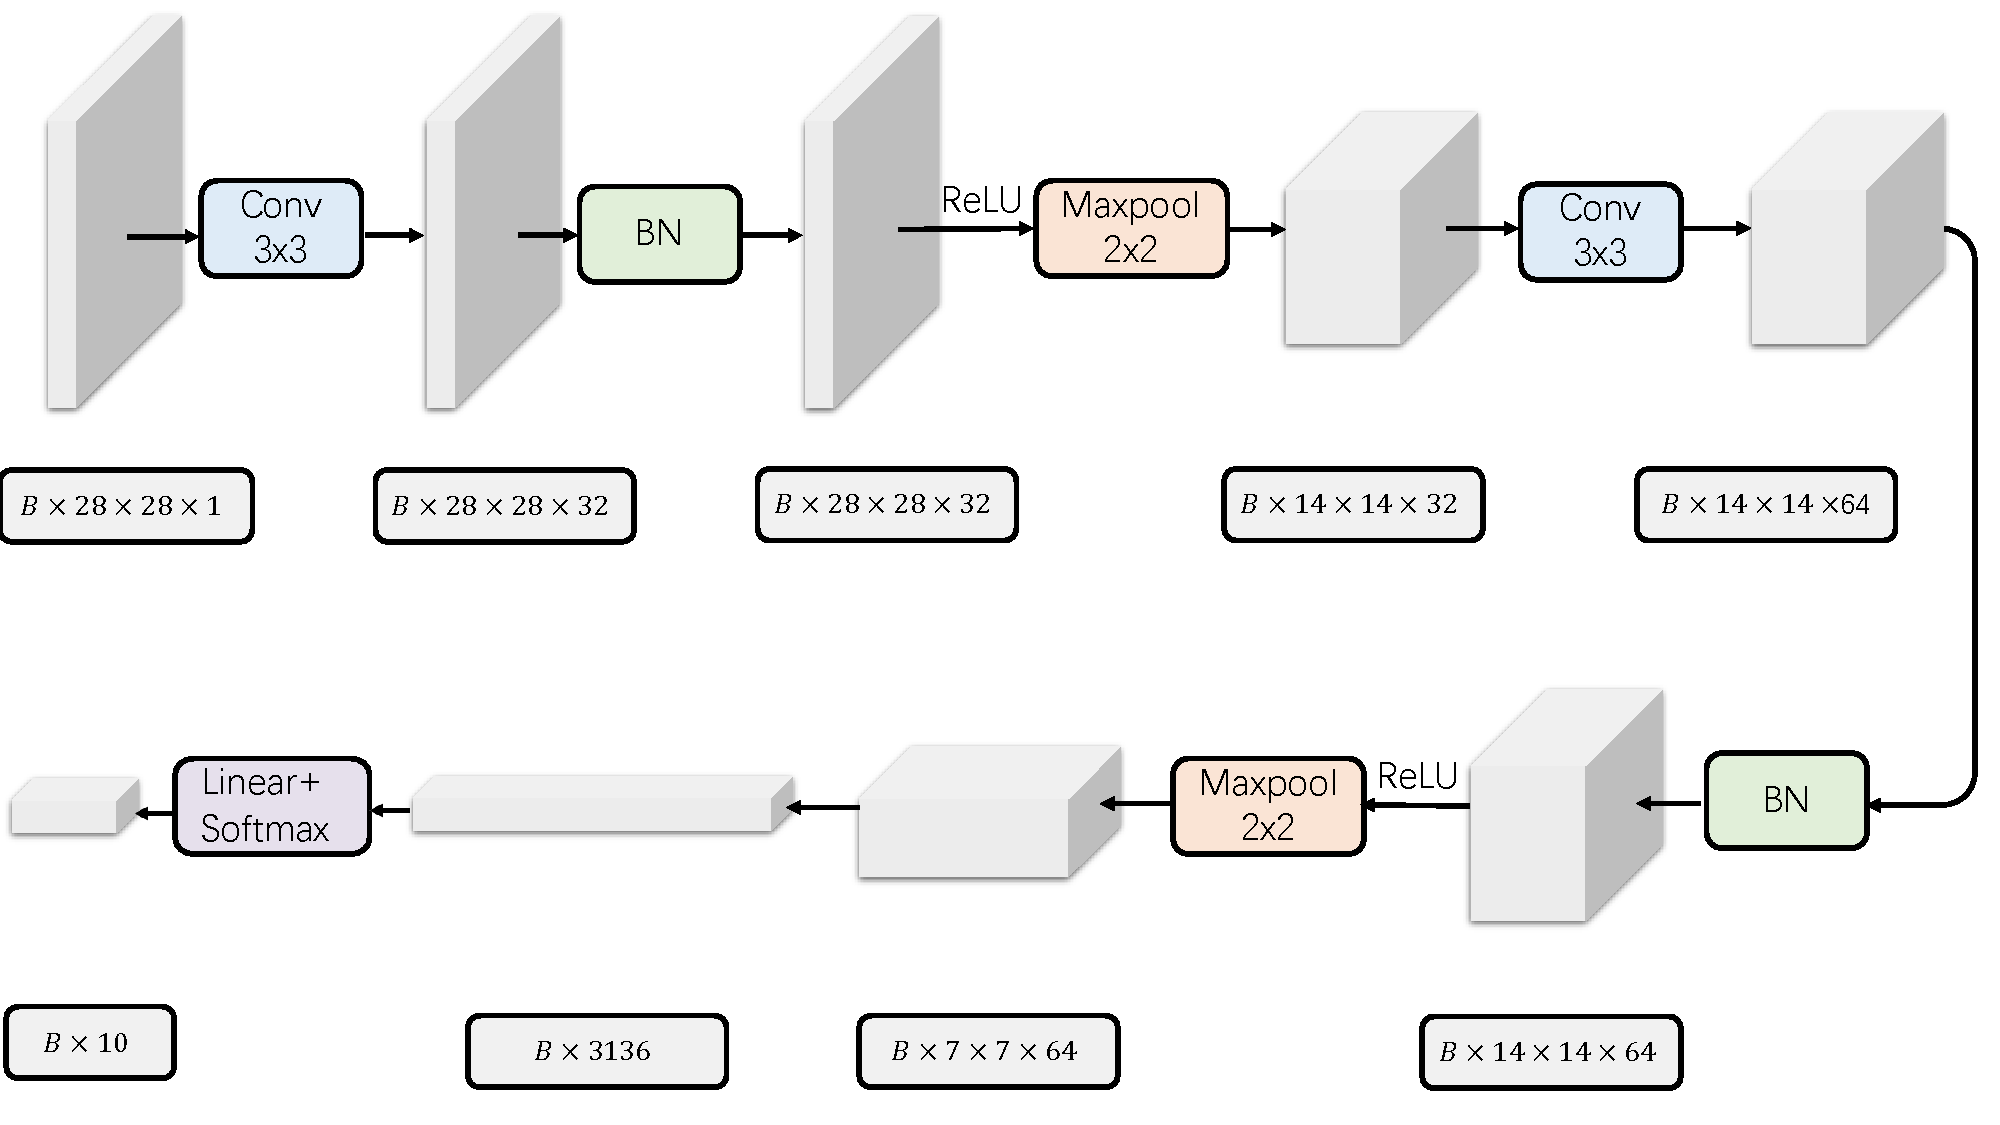
\includegraphics[width=0.8\textwidth]{cnn.pdf}
    \caption{Model diagram of self-designed CNN network for MNIST image classification task. The whole model contains 12 neural layers including the output layer.}
    \label{fig:CNN_arch}
\end{figure}

\begin{figure}[htbp]
    \centering
    \includegraphics[width=0.9\textwidth]{../images/mnist-train-loss-acc.png}
    \caption{Training loss and accuracy change figures. The left figure corresponds to the change of loss and the right one corresponds to the change of accuracy.}
    \label{fig:cnn_loss_acc}
\end{figure}

\begin{figure}[htbp]
    \centering
    \begin{subfigure}
        \centering
        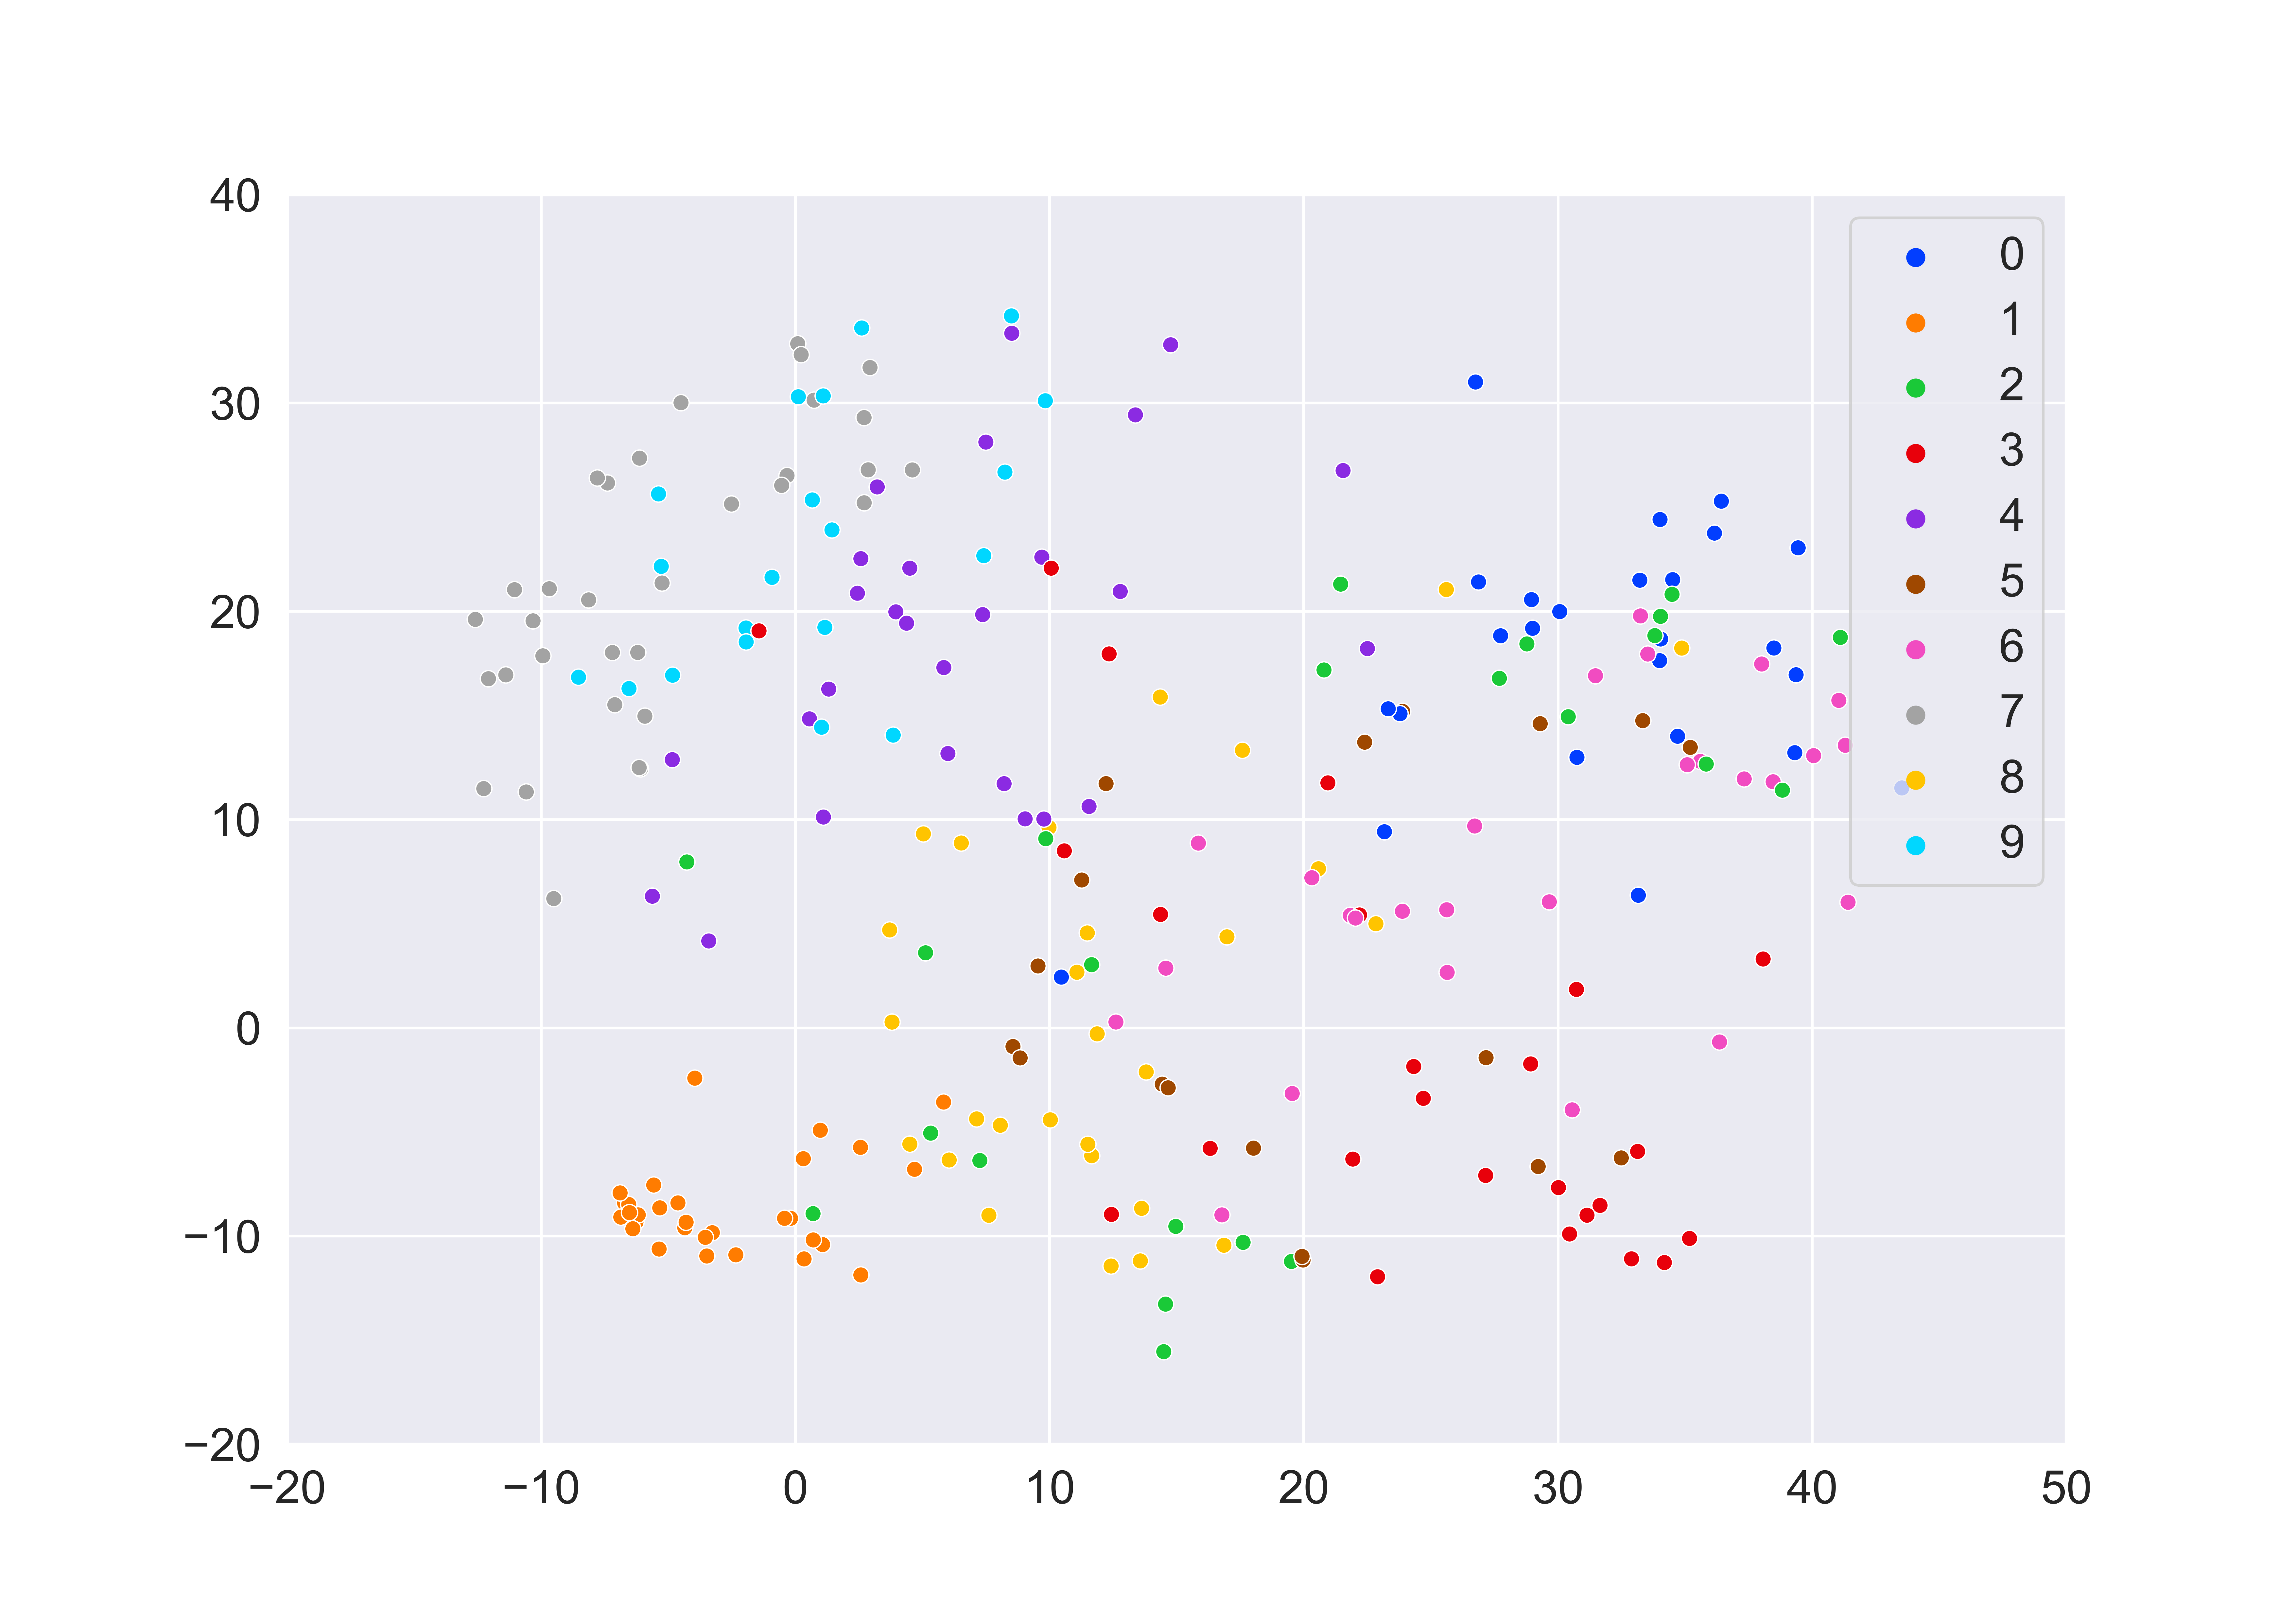
\includegraphics[width=0.32\linewidth]{../images/mnist_feature_map1_pca.png}
        % \caption{a}
        \label{fig:mnist_pca_1}
    \end{subfigure}
    % \hfill 
    \begin{subfigure}
        \centering
        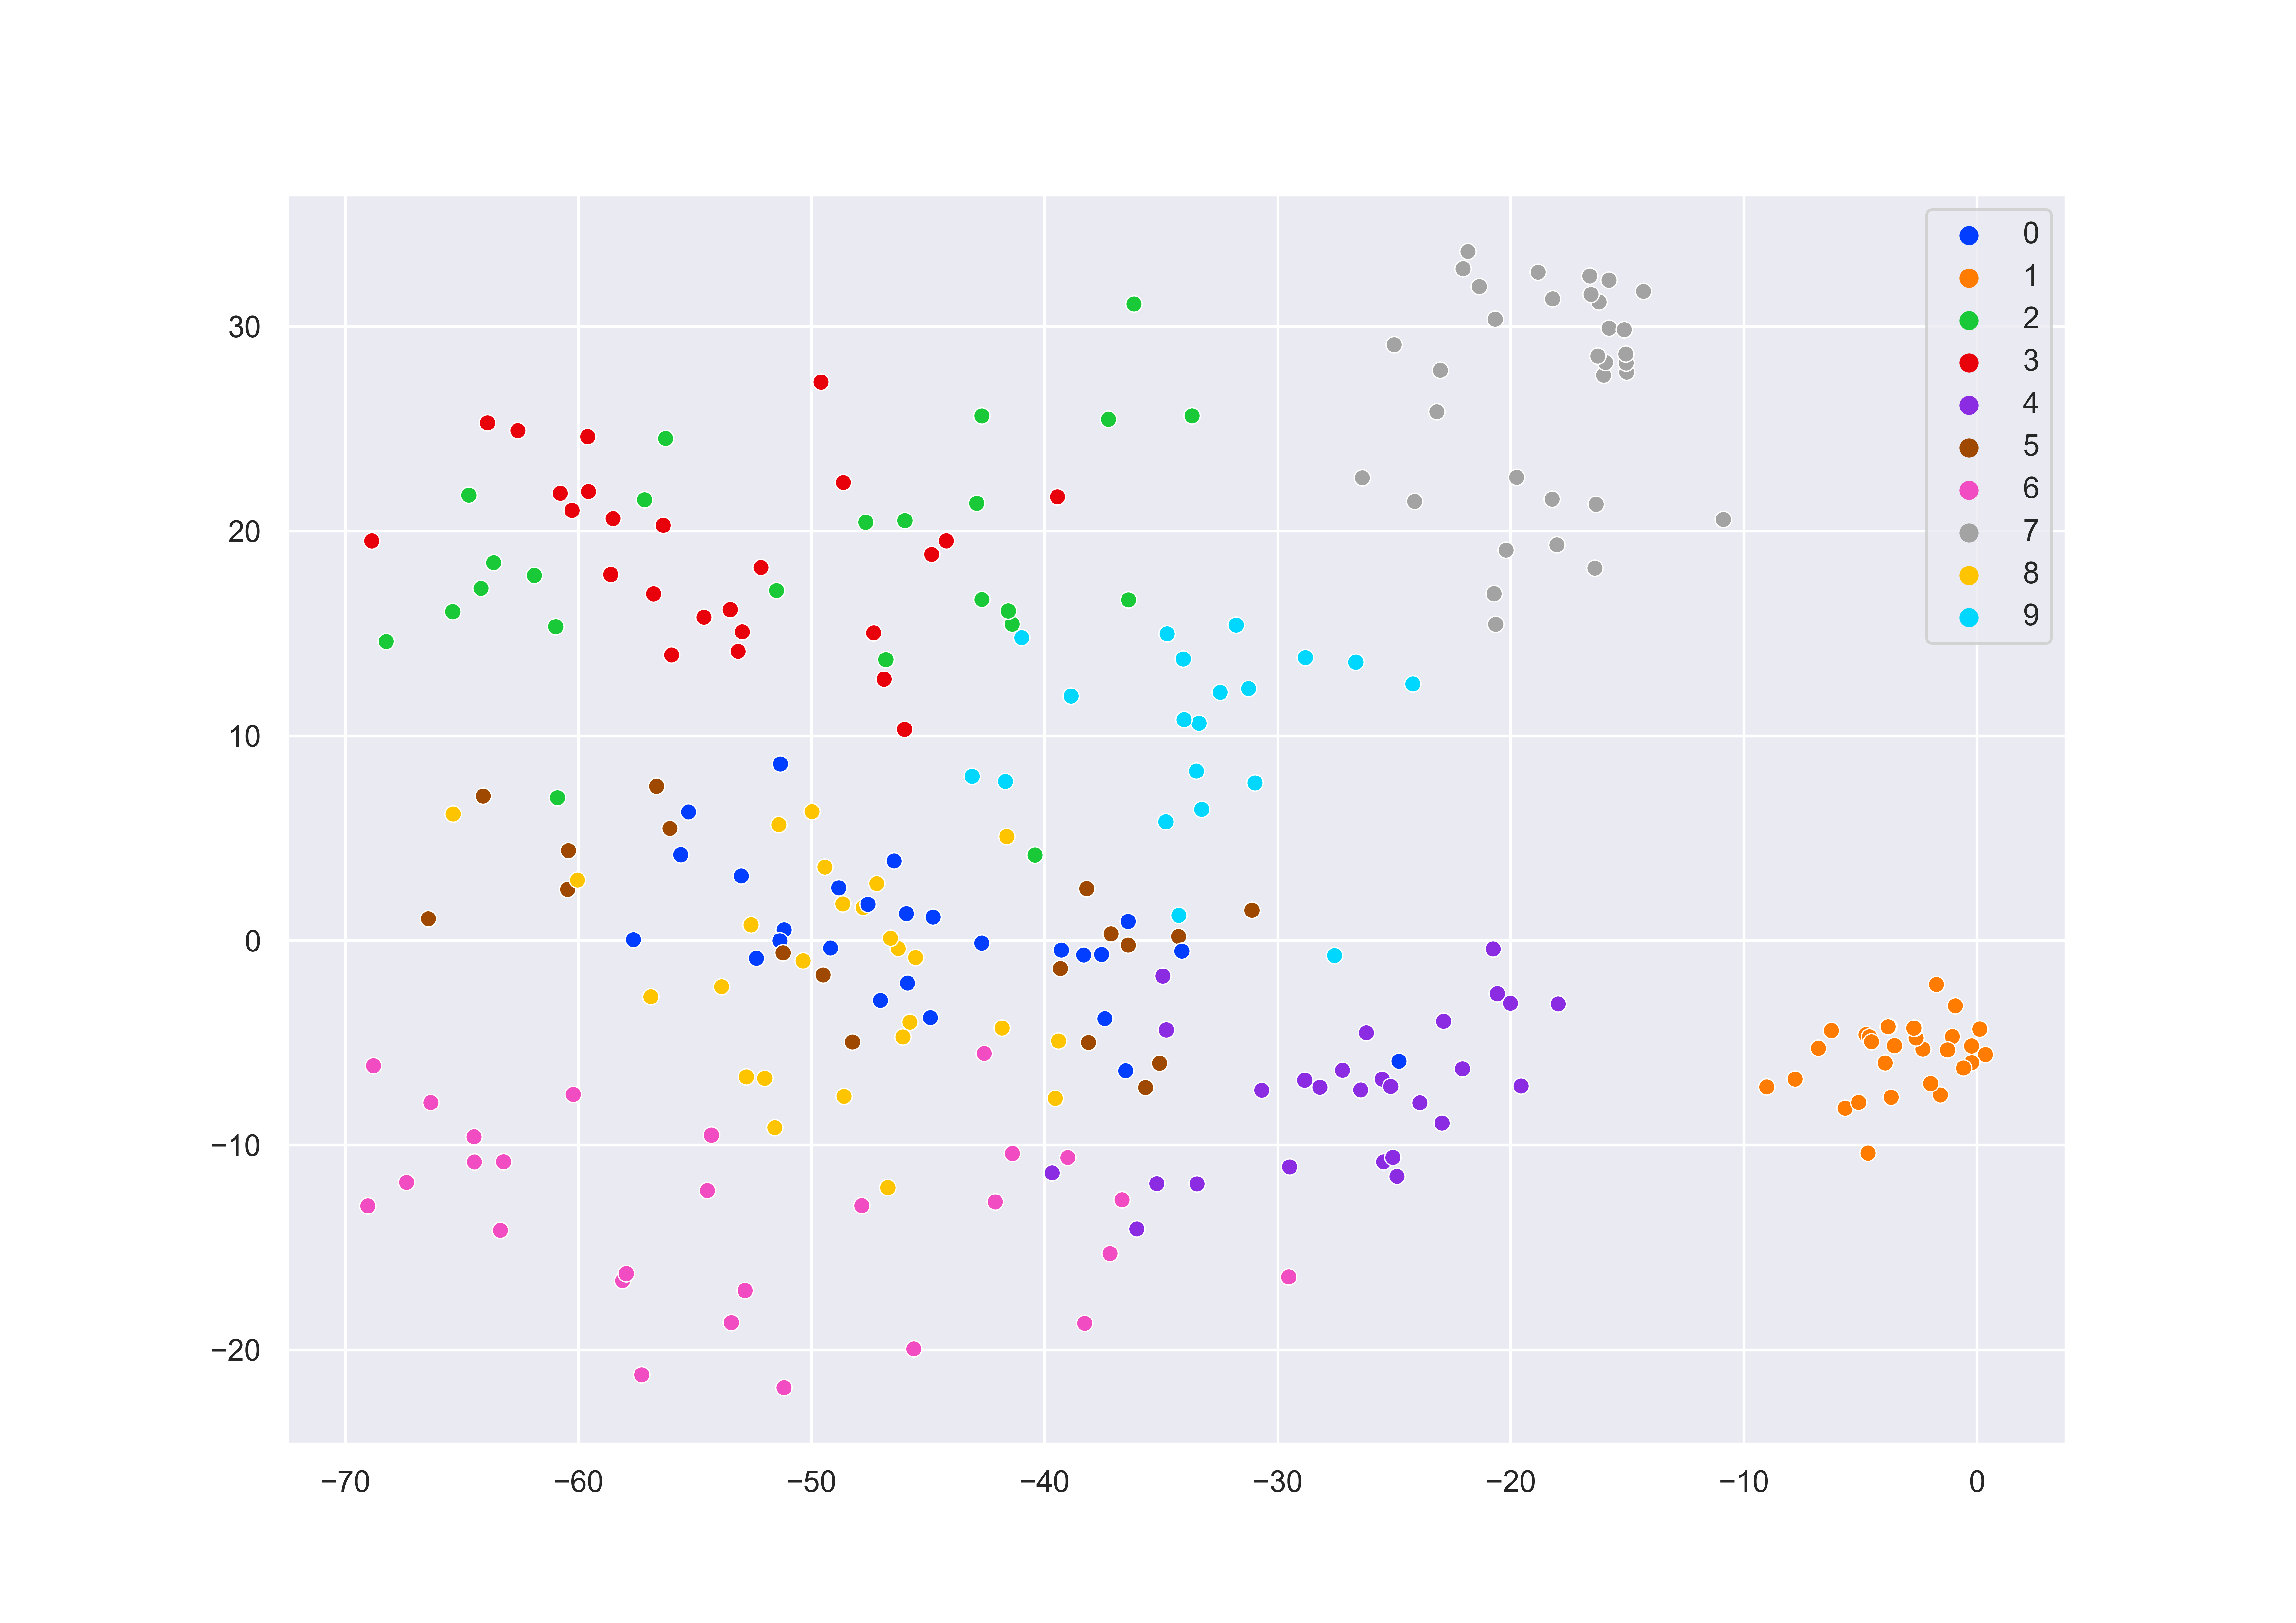
\includegraphics[width=0.32\linewidth]{../images/mnist_feature_map2_pca.png}
        % \caption{Absolute value of indivisual components of weight in ridge regression when setting $\lambda$ to 1.0.}
        \label{fig:mnist_pca_2}
    \end{subfigure}
    % \hfill 
    \begin{subfigure}
        \centering
        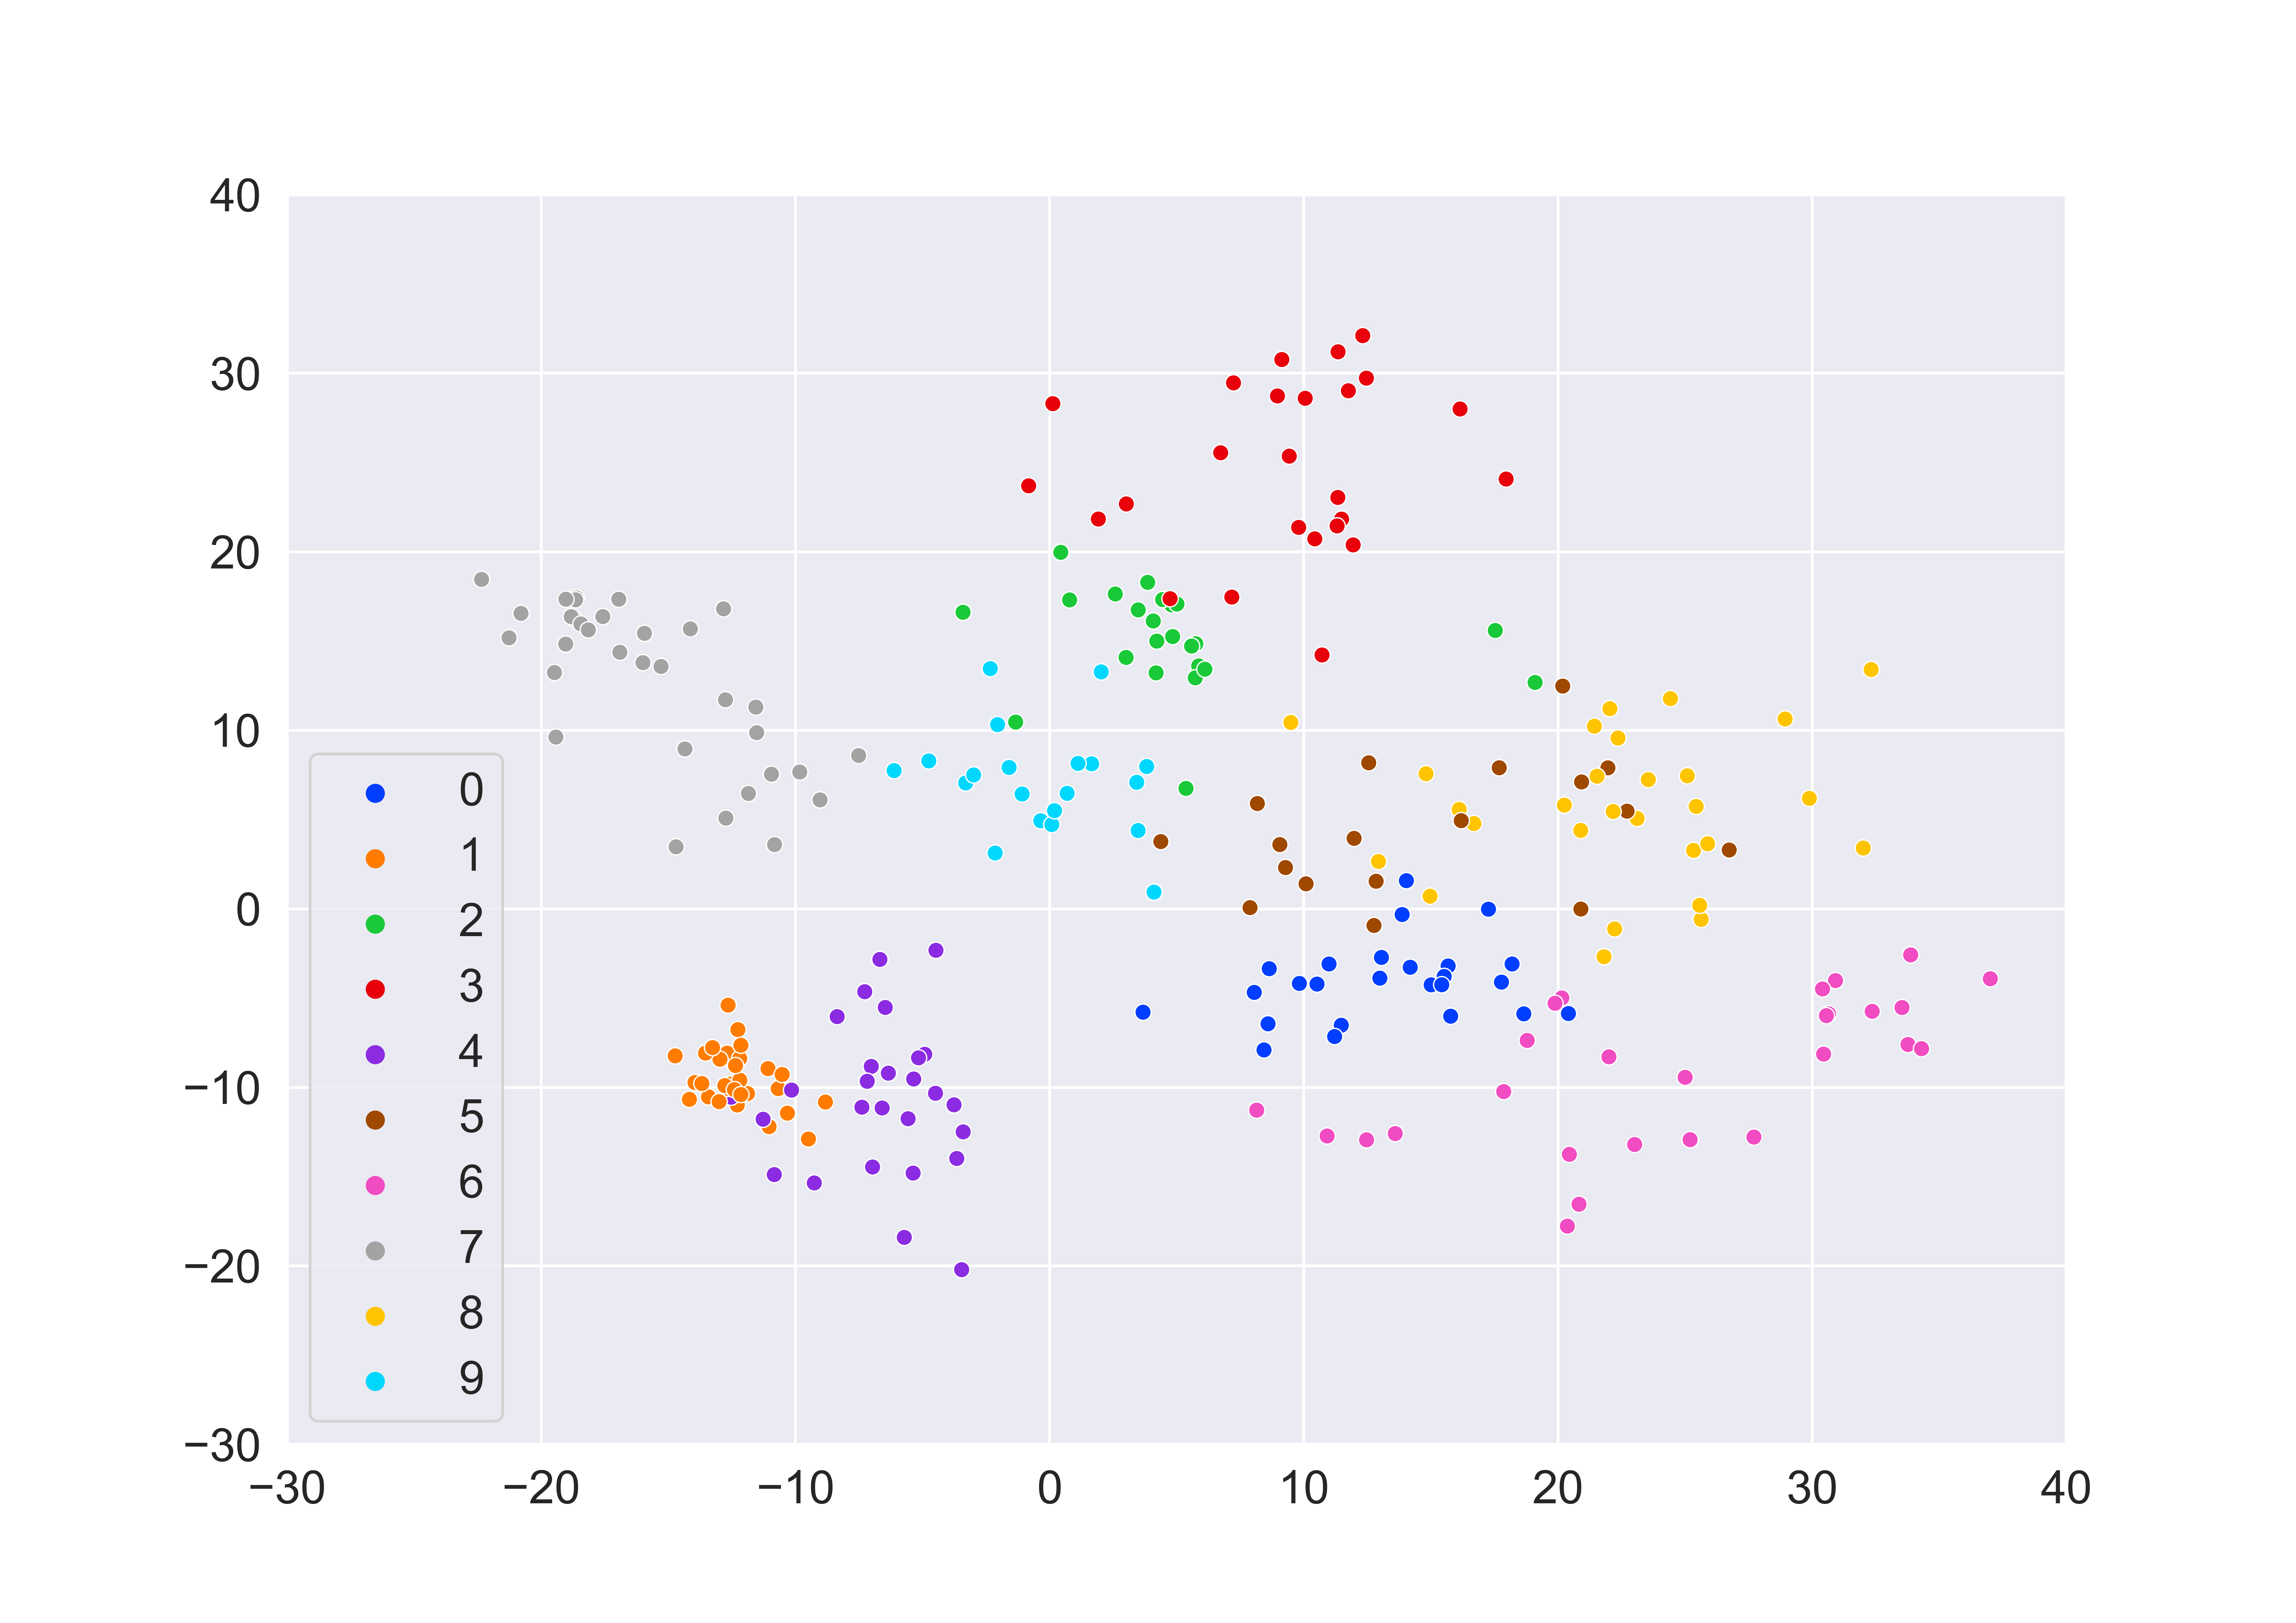
\includegraphics[width=0.32\linewidth]{../images/mnist_feature_map3_pca.png}
        % \caption{Absolute value of indivisual components of weight in ridge regression when setting $\lambda$ to 1.5.}
        \label{fig:mnist_pca_3}
    \end{subfigure}
    \caption{Visualization images of intermediate output tensors with PCA method. Left: Tensors after the first max pooling layer. Middle: Tensors after the second max pooling layer. Right: Tensors after the output linear layer.}
    \label{fig:mnist_pca}
\end{figure}

\begin{figure}[htbp]
    \centering
    \begin{subfigure}
        \centering
        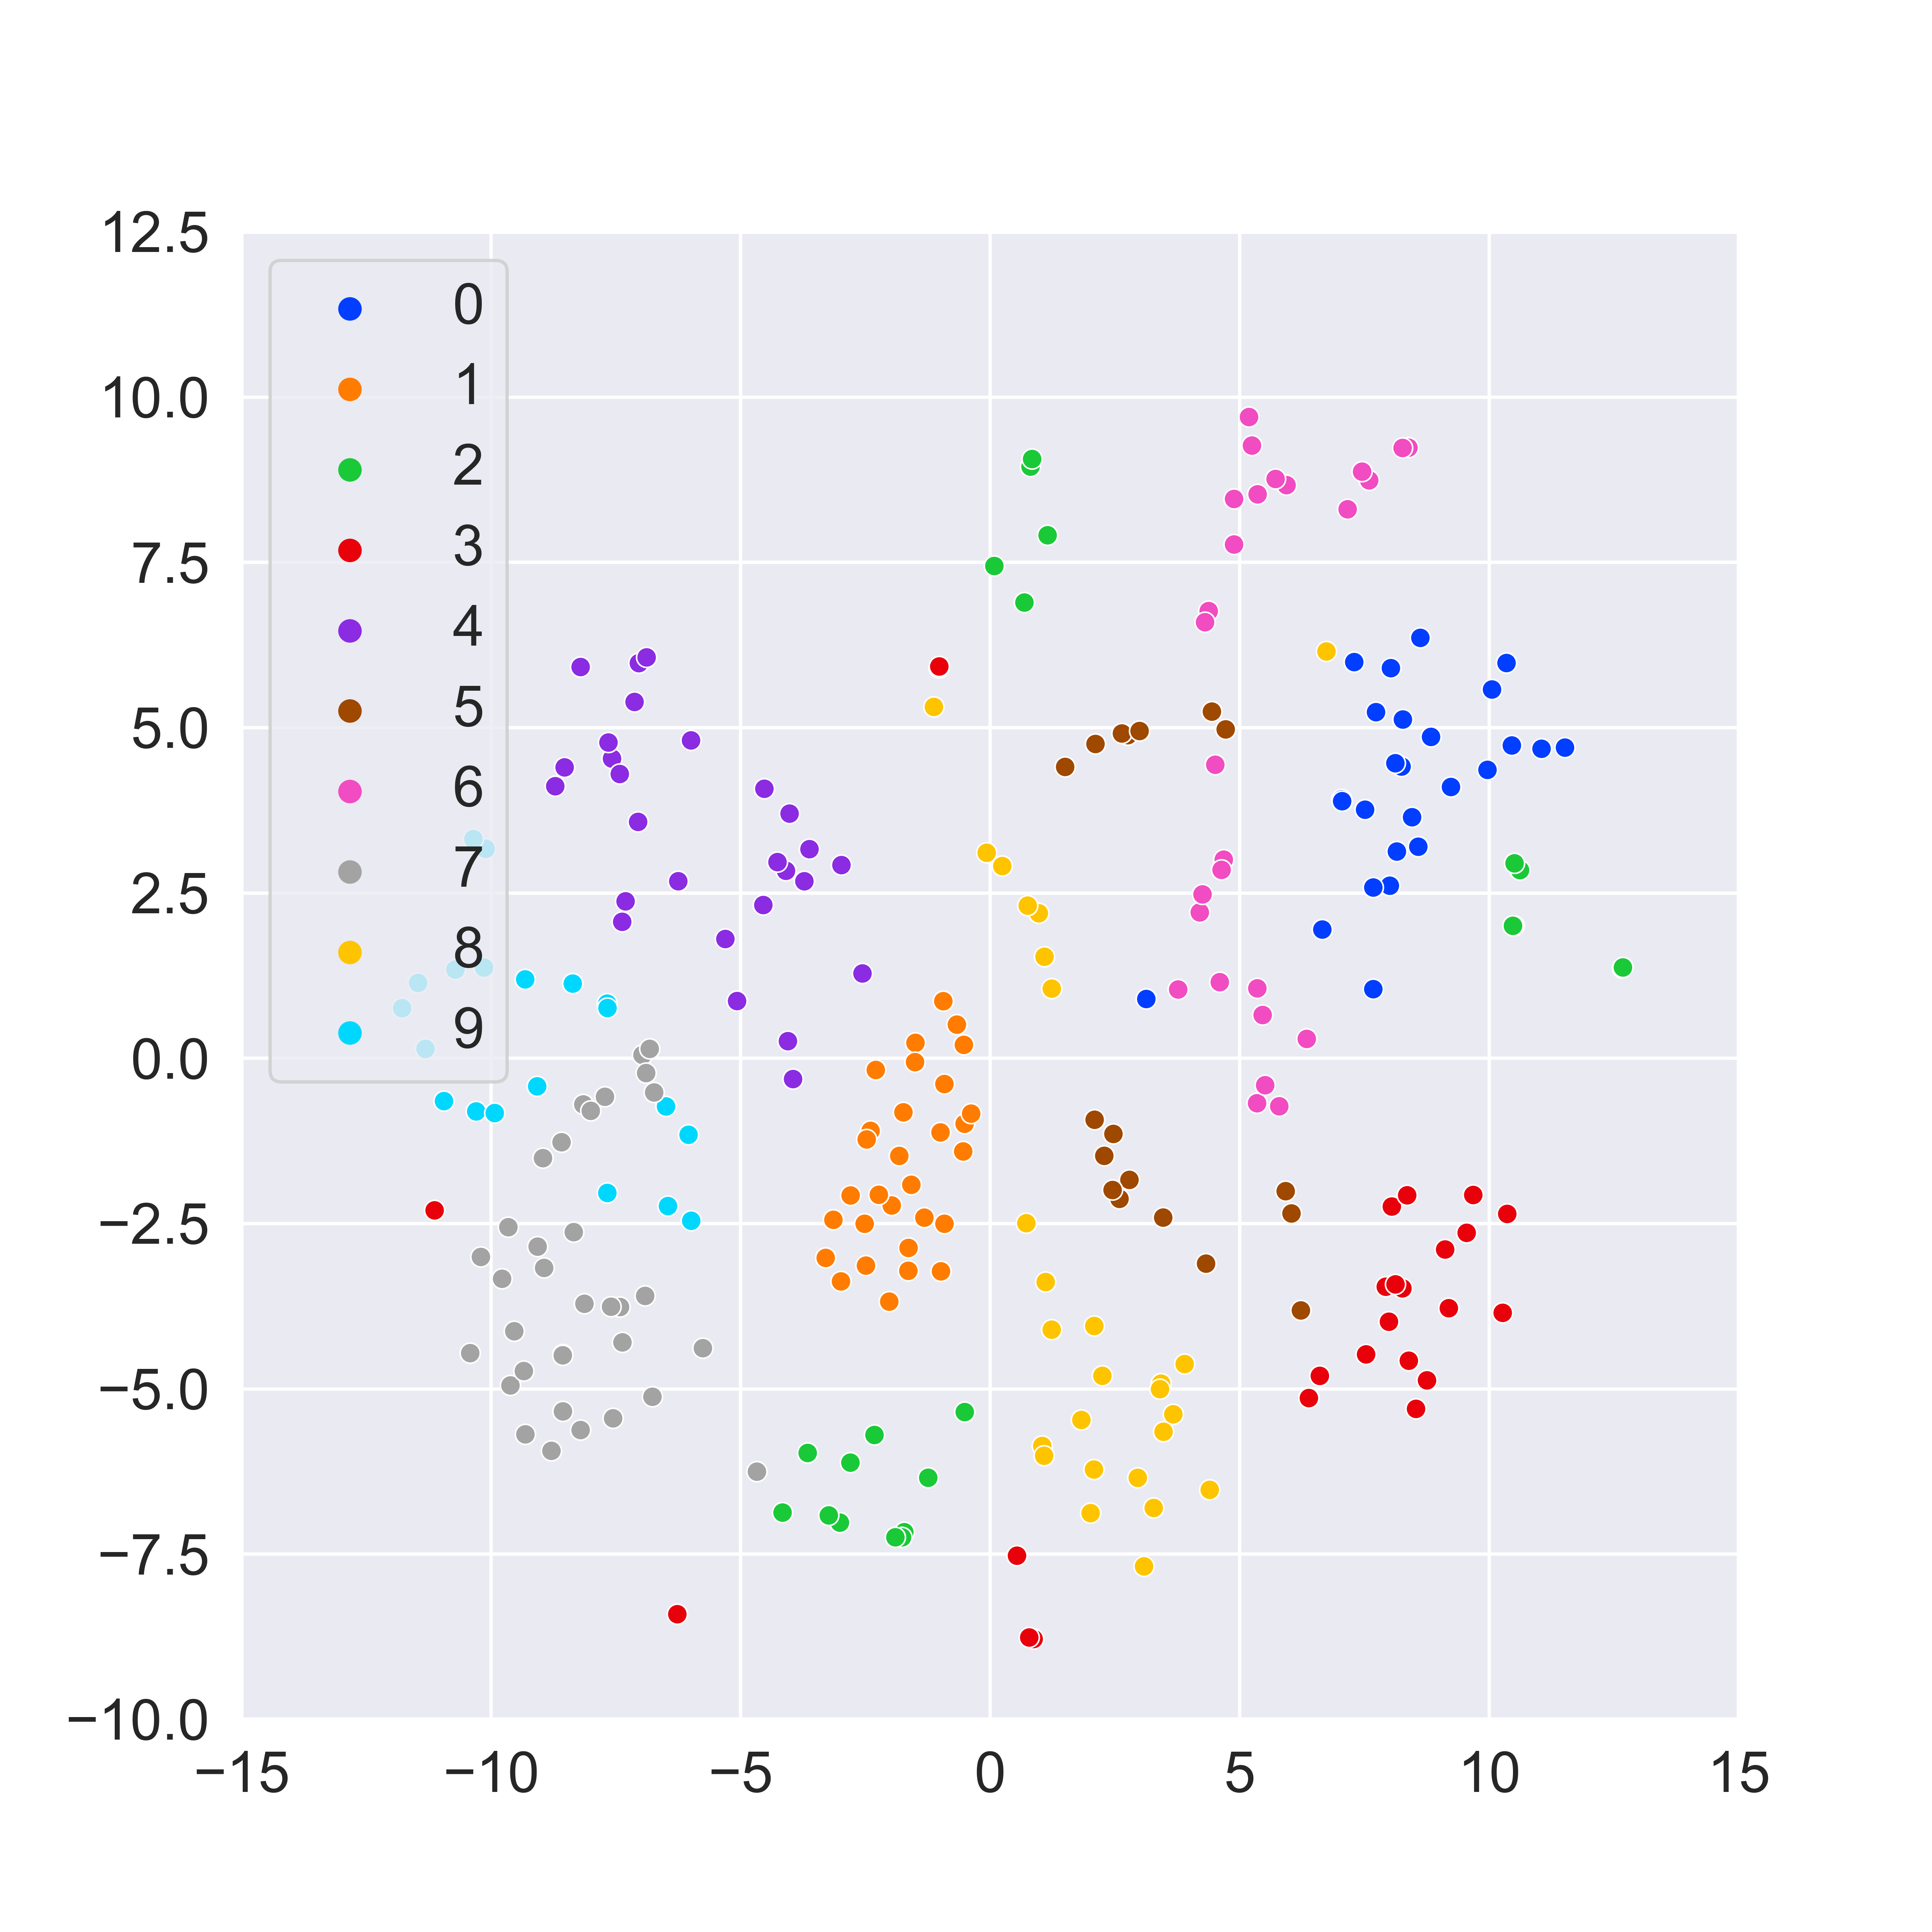
\includegraphics[width=0.32\linewidth]{../images/mnist_feature_map1_tsne.png}
        % \caption{a}
        \label{fig:mnist_tSNE_1}
    \end{subfigure}
    % \hfill 
    \begin{subfigure}
        \centering
        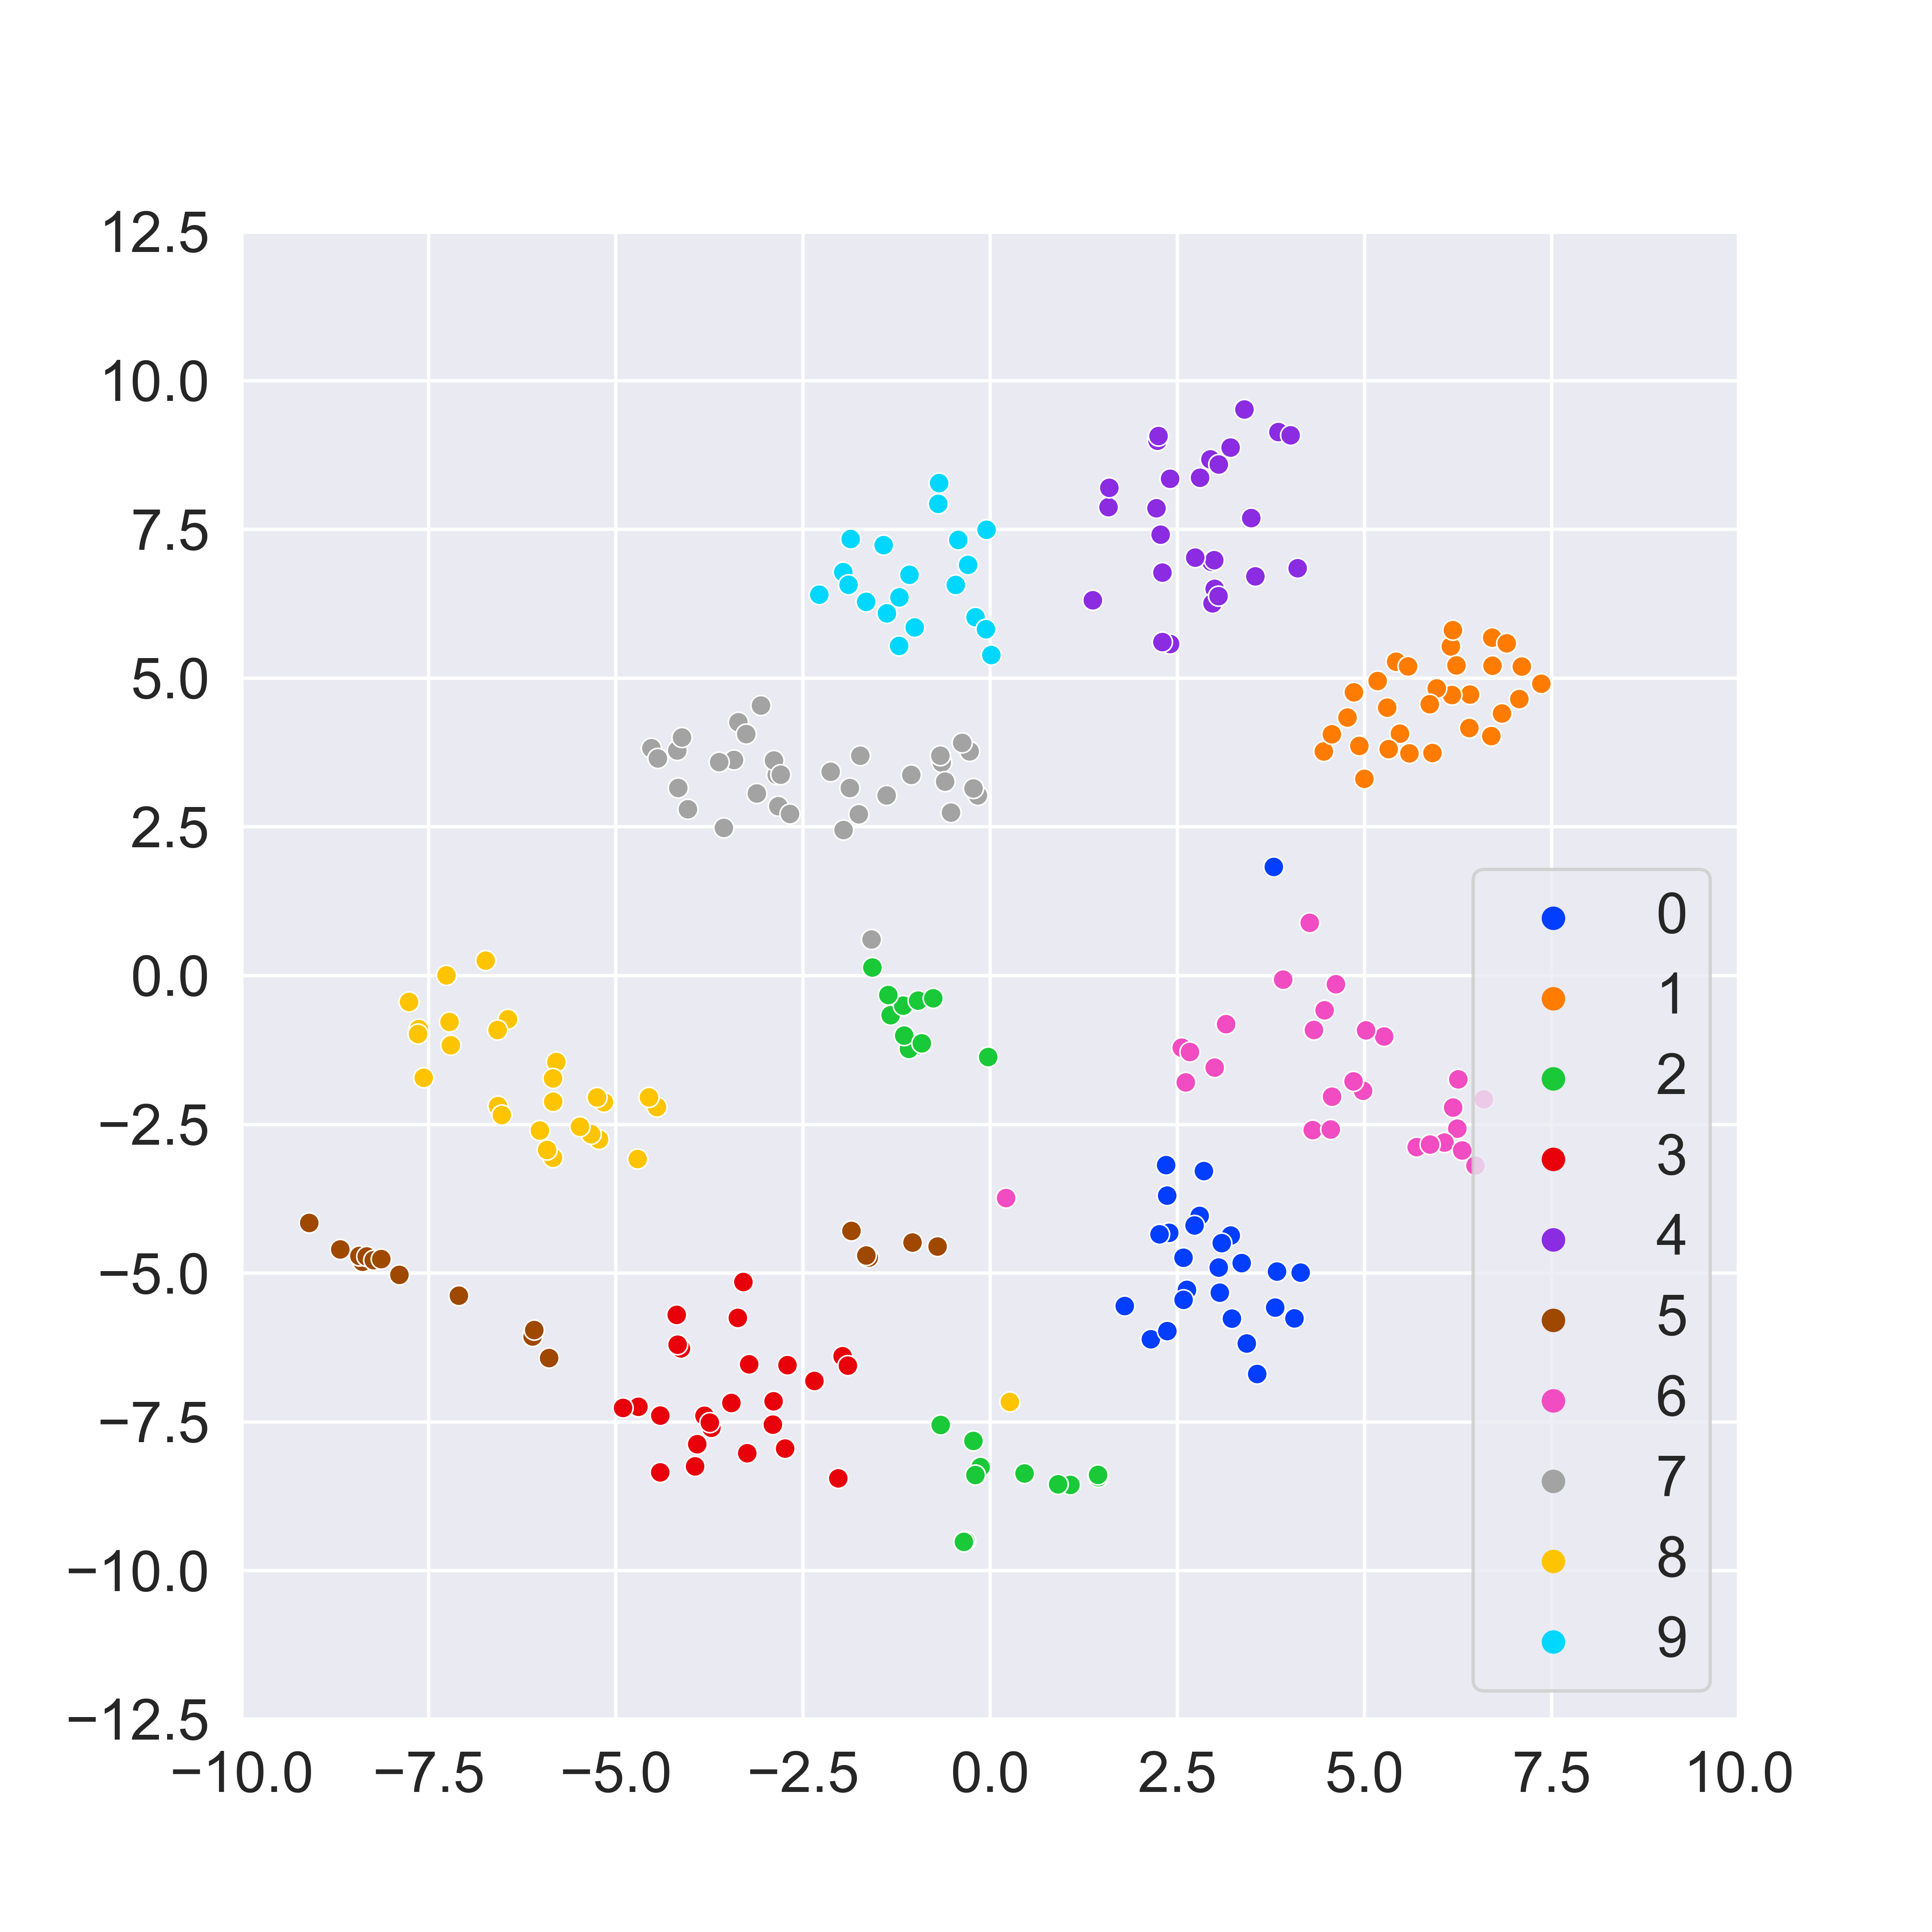
\includegraphics[width=0.32\linewidth]{../images/mnist_feature_map2_tsne.png}
        % \caption{Absolute value of indivisual components of weight in ridge regression when setting $\lambda$ to 1.0.}
        \label{fig:mnist_tSNE_2}
    \end{subfigure}
    % \hfill 
    \begin{subfigure}
        \centering
        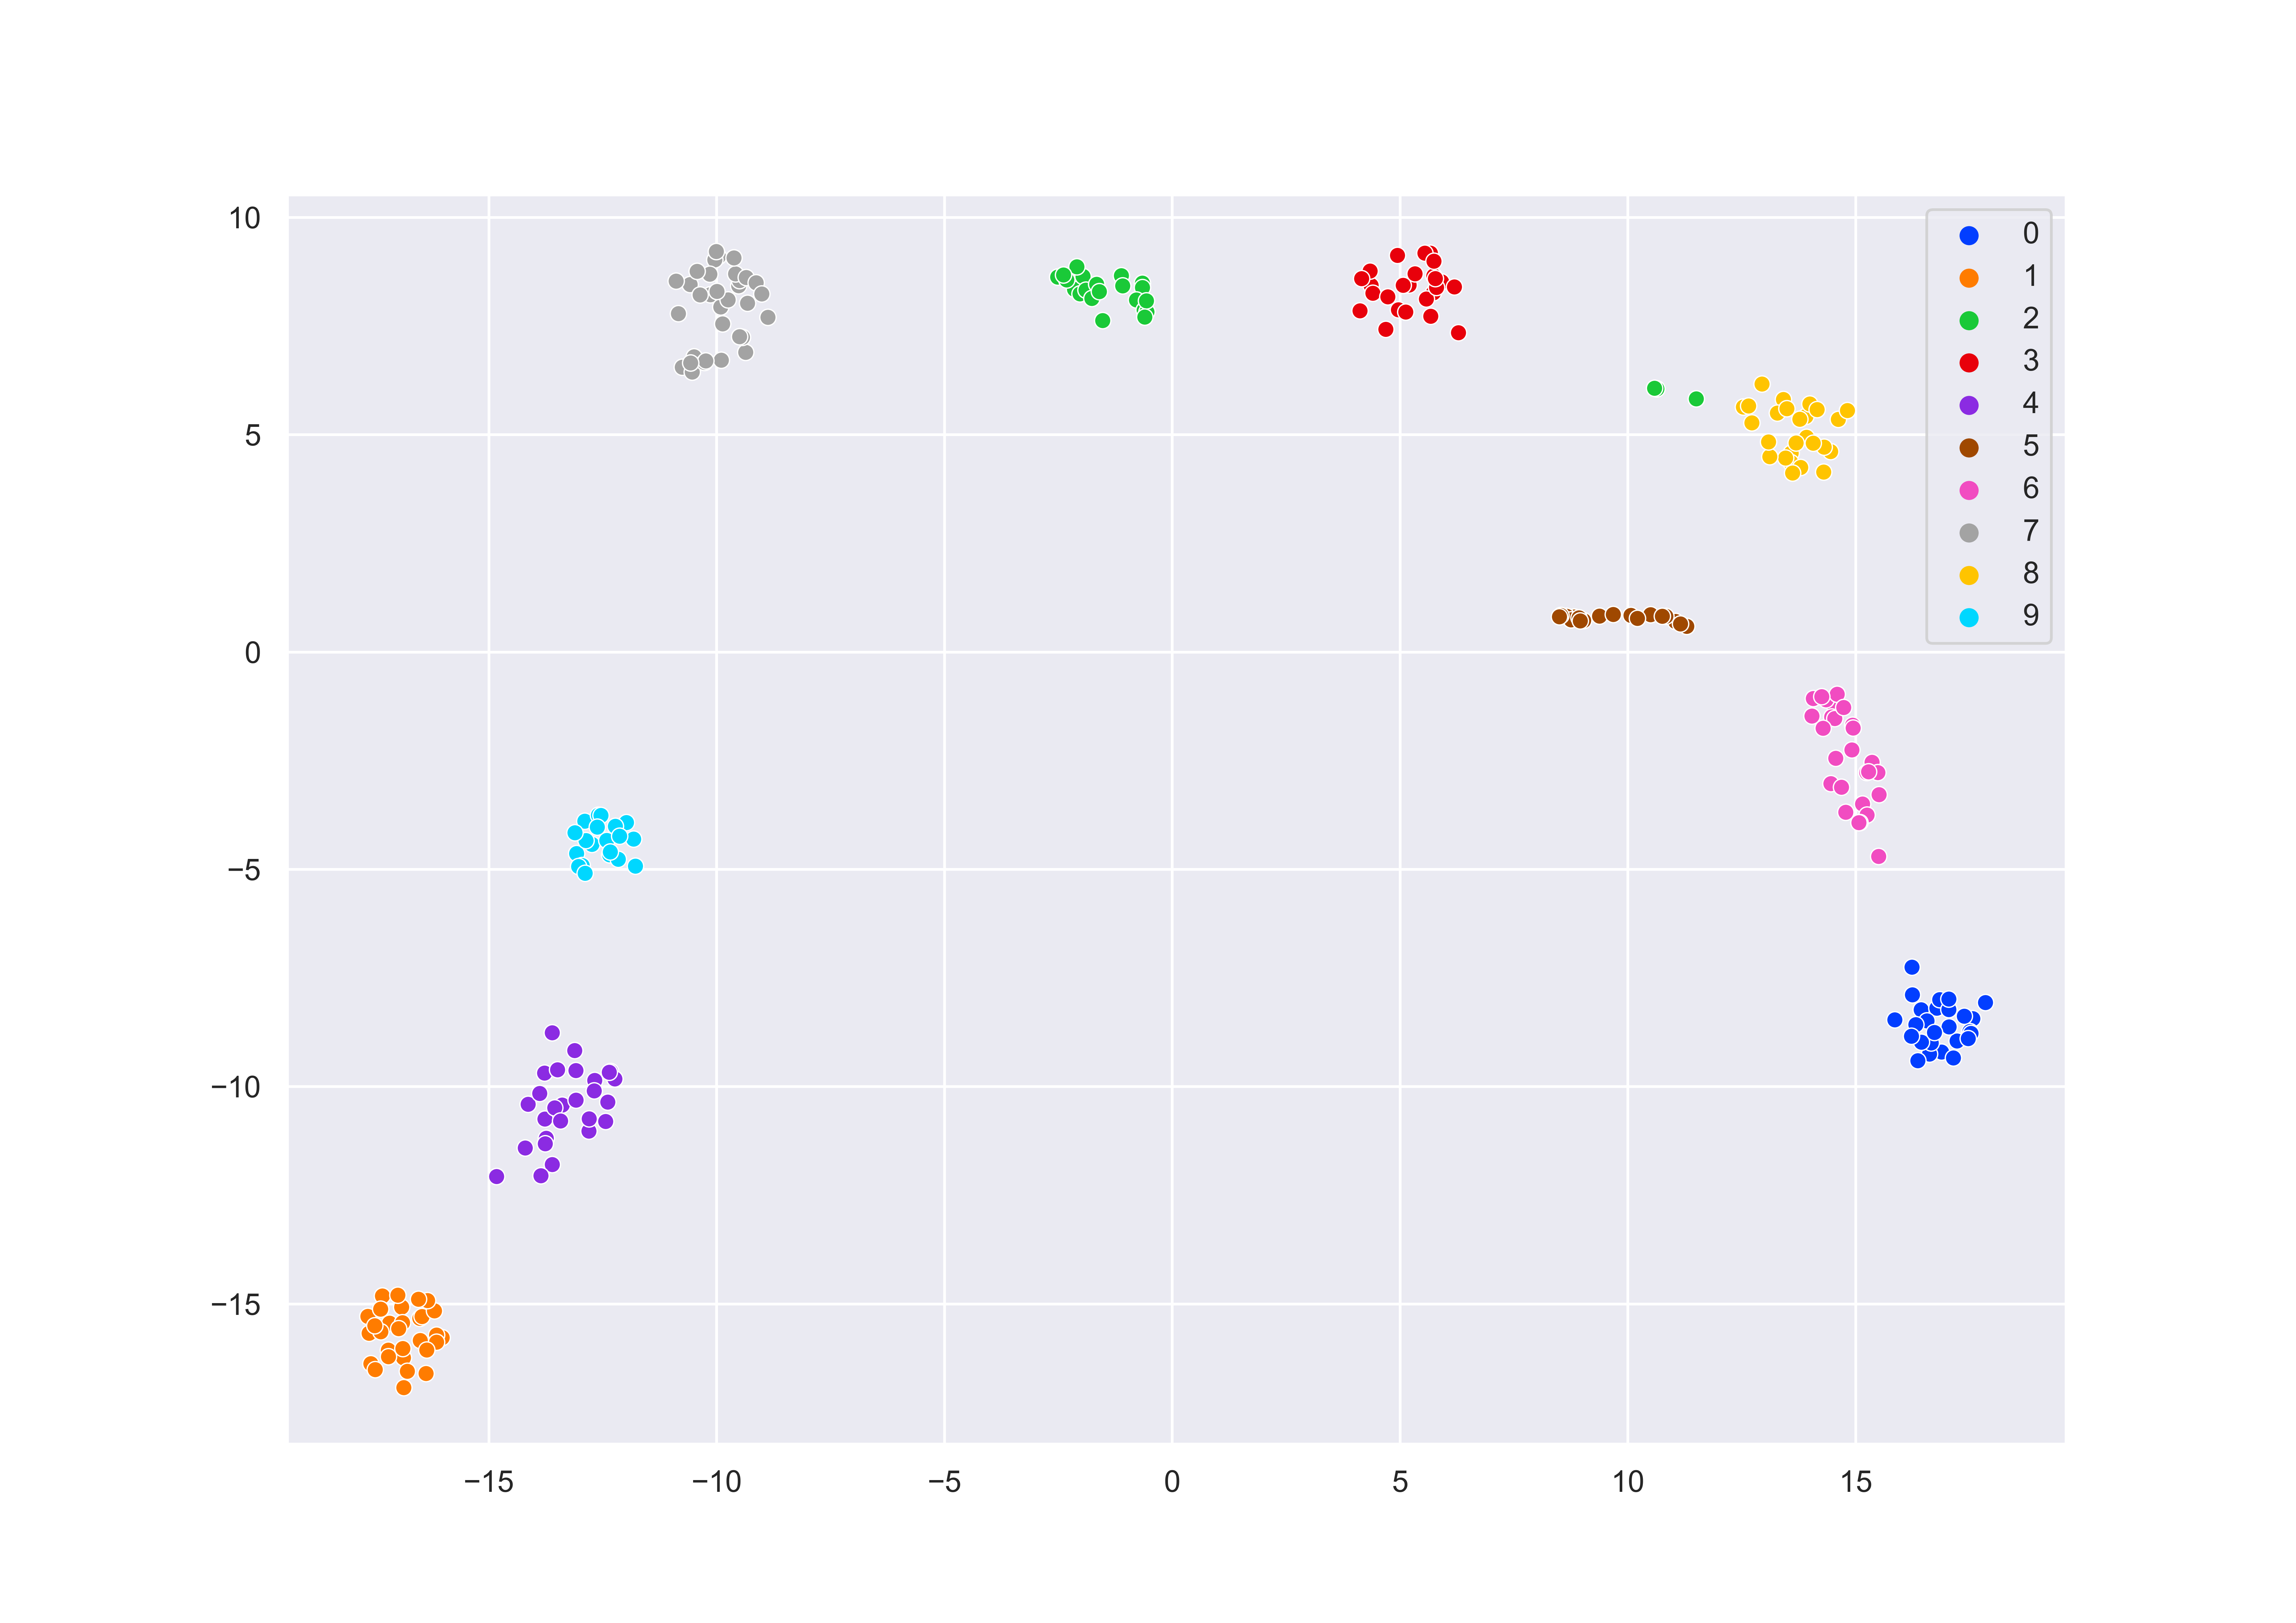
\includegraphics[width=0.32\linewidth]{../images/mnist_feature_map3_tsne.png}
        % \caption{Absolute value of indivisual components of weight in ridge regression when setting $\lambda$ to 1.5.}
        \label{fig:mnist_tSNE_3}
    \end{subfigure}
    \caption{Visualization images of intermediate output tensors with t-SNE method. Left: Tensors after the first max pooling layer. Middle: Tensors after the second max pooling layer. Right: Tensors after the output linear layer.}
    \label{fig:mnist_tsne}
\end{figure}

\section{Image Classification}
\subsection{Model \& Hyperparameters}
I design a 2-layer CNN models with an additional linear and softmax layer. The architecture can be interpreted in Fig.~\ref{fig:CNN_arch}. 
I set the batch size to 256 so as to maintain the high capability of batch normalization layer. 
The learning rate is set to 0.001 and the dropout rate is set to 0.1.
I train the whole model for 30 epochs and select the checkpoint with best binary cross entropy loss for evaluation on test set.

\subsection{Experiment Results}
The selected checkpoint can achieve $99.39\%$ accuracy in test set. The loss and accuracy change figures of self-designed CNN model are depicted in Fig.~\ref{fig:cnn_loss_acc}. It can be seen that the change is smooth, which proves that the hyperparameters are well-set and does not require more tuning steps.

Besides, I output the tensor after the first pooling layer, the tensor after the second pooling layer and the tensor after the output linear layer. 
And then I use PCA and t-SNE to respectively visualize them in order to see what my model has learned during training.
Their corresponding results are depicted in Fig.~\ref{fig:mnist_pca} and Fig.~\ref{fig:mnist_tsne}, respectively.
It can be seen that the first tensor cannot distinguish well each images but after the second CNN layer, my model has learned to distinguish each image with high accuracy.

% \subsection{Linear Regression}
% Given an input sample set $X\in\mathbb{R}^{n\times d}$, where $n$ is the number of samples and $d$ is the dimensionality of feature space, linear regression often random initializes a weight matrix $W\in\mathbb{R}^{d}$ and use gradient descent to update its value.
% In detail, to predict the output value, linear regression uses such formula to predict an output in matrix form:
% \begin{equation}
%     \label{eq:linear_regression}
%     \hat{Y}=XW
% \end{equation}
% Once predicted output is obtained, the error~(known as loss value) between ground truth and predicted value can be computed via MSE loss:
% \begin{equation}
%     \label{mse_loss}
%     \mathcal{L}=\frac{1}{2}\left\Vert Y^*-\hat{Y} \right\Vert_2^2
% \end{equation}
% where $Y^*\in\mathbb{R}^{n}$ is the ground truth value. First compute its gradient with respect to $W$ as:
% \begin{equation}
%     \label{eq:linear_gradient}
%     \frac{\partial \mathcal{L}}{\partial W}=-X^\top(Y-XW)
% \end{equation}
% Therefore, values of $W$ can be updated given appropriate learning rate $\eta$ as:
% \begin{equation}
%     \label{eq:update}
%     W=W-\eta \frac{\partial \mathcal{L}}{\partial W}
% \end{equation}
% \subsection{Ridge Regression}
% The predicted output value is the same as Eq.~\ref{eq:linear_regression}. However, to avoid over-fitting and gradient explosion, a regularization term with suitable hyperparameter $\lambda$ is added in the loss function:
% \begin{equation}
%     \label{mse_l2}
%     \mathcal{L}=\frac{1}{2}\left\Vert Y^*-\hat{Y} \right\Vert_2^2+\frac{\lambda}{2}\left\Vert W \right\Vert_2
% \end{equation}
% Using this setting, the gradient can be computed as:
% \begin{equation}
%     \frac{\partial \mathcal{L}}{\partial W}=-X^\top(Y-XW)+\lambda W
% \end{equation}
% After computing the gradient value, Eq.~\ref{eq:update} can be used to update $W$.

% \subsection{Lasso Regression}
% The predicted output value is the same as Eq.~\ref{eq:linear_regression}. However, to avoid any exorbitant value in $W$, a regularization term with suitable hyperparameter $\lambda$ is again added in the loss function:
% \begin{equation}
%     \label{mse_l2}
%     \mathcal{L}=\frac{1}{2}\left\Vert Y^*-\hat{Y} \right\Vert_2^2+\lambda\left\Vert W \right\Vert_1
% \end{equation}
% Using this setting, the gradient can be computed as:
% \begin{equation}
%     \frac{\partial \mathcal{L}}{\partial W}=-X^\top(Y-XW)+\lambda \cdot \mathrm{sign}(W)
% \end{equation}
% After computing the gradient value, Eq.~\ref{eq:update} can be used to update $W$.

% \subsection{Kernel Regression}
% Different from above methods, Kernel Regression projects each sample to higher dimension space, which is beneficial for classification. 
% To predict value, I set the kernel function as RBF kernel and set the hyperparameter $\gamma$ to $0.5$: $\texttt{Ker}(\boldsymbol{x,x'})=e^{\gamma \left\Vert \boldsymbol{x-x'}\right\Vert}$. 
% And use matrix form to construct a kenel sample $K\in\mathbb{R}^{n\times n}$, where $K_{ij}=\texttt{Ker}(\boldsymbol{X_i, X_j})$ 
% For each sample, I define a learnable parameter $c\in\mathbb{R}^{n}$. 
% Considering that the weight $W=\phi(X)^\top c$ can not be obtained from $c$, I report the absolute value of each component of $c$ in Fig.~\ref{fig:kernel_component}.

% In detail, the predicted value can be computed as:
% \begin{equation}
%     \label{kernel_output}
%     \hat{Y}=Kc
% \end{equation}

% The loss value can be computed with a hyperparameter $\lambda$ similar to Eq.~\ref{mse_l2} as:
% \begin{equation}
%     \label{mse_kernel}
%     \mathcal{L}=\frac{1}{2}\left\Vert Y^*-\hat{Y} \right\Vert_2^2+\frac{1}{2}\lambda c^\top K c
% \end{equation}
% The gradient with respect to $W$ can be computed as:
% \begin{equation}
%     \frac{\partial \mathcal{L}}{\partial W}=-K^\top(Y^*-Kc)+\lambda Kc
% \end{equation}
% After computing the gradient value, Eq.~\ref{eq:update} can be used to update $W$.

% \section{Test Error with Different Hyperparameters}
% In this section, I report the test error of different methods in the test set. 
% I follow the instructions of the dataset to apply $\ln(x+1)$ to each area value.
% After each algorithm converges, I directly compute the absolute test error of the logarithm value instead of original value.
% For Ridge Regression, Lasso Regression and Kernel Regression, I test three different $\lambda$ values~($0.5,1.0,1.5$) and report their test errors, respectively.
% I train all models with learning rate $1\times 10^{-5}$ for $1000$ epochs.
% The results are shown in Table.~\ref{tab:test_error}.


% \begin{table}[!htbp]
%     \centering
%     \caption{Test error with different methods. For ridge regression, lasso regression and kernel regression, I report their corresponding test error respectively.}
%     \begin{tabular}{c|c|c}
%         \toprule
%         \multicolumn{1}{l|}{Model Setting} & \multicolumn{1}{l|}{$\lambda$} & \multicolumn{1}{l}{Test error} \\
%         \midrule
%         \multicolumn{1}{l|}{Linear Regression} & -     & 214.514 \\
%         \midrule
%         \multirow{3}[2]{*}{Ridge Regression} & 0.5   & 175.675 \\
%               & 1.0   & 153.267 \\
%               & 1.5   & 195.234 \\
%         \midrule
%         \multirow{3}[2]{*}{Lasso Regression} & 0.5   & 176.417 \\
%               & 1.0   & 204.963 \\
%               & 1.5   & 147.916 \\
%         \midrule
%         \multirow{3}[2]{*}{Kernel Regression} & 0.5   & 171.773 \\
%               & 1.0   & 193.679 \\
%               & 1.5   & 196.902 \\
%         \bottomrule
%         \end{tabular}%
%     \label{tab:test_error}%
%   \end{table}%

% \section{Absolute Value of Each Weight}
% In this section, I follow the instruction of the task to plot the absolute value of each individual component of weight matrix in descending order. 
% The absolute value figure of \textbf{lienar regression} is presented in Fig.~\ref{fig:linear_component}.
% The absolute value figure of \textbf{ridge regression} is presented in Fig.~\ref{fig:ridge_component}.
% The absolute value figure of \textbf{lasso regression} is presented in Fig.~\ref{fig:lasso_component}.
% The absolute value figure of \textbf{kernel regression} is presented in Fig.~\ref{fig:kernel_component}.
% \begin{figure}[htbp]
%     \centering
    
%     \includegraphics[width=0.7\linewidth]{../img/weight_vanilla_regression.png}
%     \caption{Absolute value of indivisual components of weight in linear regression.}
%     \label{fig:linear_component}
% \end{figure}
% \begin{figure}[htbp]
%     \centering
%     \begin{subfigure}
%         \centering
%         \includegraphics[width=0.32\linewidth]{../img/weight_ridge_regression_0.5.png}
%         % \caption{Absolute value of indivisual components of weight in ridge regression when setting $\lambda$ to 0.5.}
%         \label{fig:ridge_component_0.5}
%     \end{subfigure}
%     % \hfill 
%     \begin{subfigure}
%         \centering
%         \includegraphics[width=0.32\linewidth]{../img/weight_ridge_regression_1.0.png}
%         % \caption{Absolute value of indivisual components of weight in ridge regression when setting $\lambda$ to 1.0.}
%         \label{fig:ridge_component_1.0}
%     \end{subfigure}
%     % \hfill 
%     \begin{subfigure}
%         \centering
%         \includegraphics[width=0.32\linewidth]{../img/weight_ridge_regression_1.5.png}
%         % \caption{Absolute value of indivisual components of weight in ridge regression when setting $\lambda$ to 1.5.}
%         \label{fig:ridge_component_1.5}
%     \end{subfigure}
%     \caption{Absolute value of indivisual components of weight in ridge regression when setting $\lambda$ to $0.5,1.0,1.5$ respectively. Figures are sorted from left to right according to corresponding $\lambda$ value.}
%     \label{fig:ridge_component}
% \end{figure}
% \begin{figure}[htbp]
%     \centering
%     \begin{subfigure}
%         \centering
%         \includegraphics[width=0.32\linewidth]{../img/weight_lasso_regression_0.5.png}
%         % \caption{Absolute value of indivisual components of weight in ridge regression when setting $\lambda$ to 0.5.}
%         \label{fig:lasso_component_0.5}
%     \end{subfigure}
%     % \hfill 
%     \begin{subfigure}
%         \centering
%         \includegraphics[width=0.32\linewidth]{../img/weight_lasso_regression_1.0.png}
%         % \caption{Absolute value of indivisual components of weight in ridge regression when setting $\lambda$ to 1.0.}
%         \label{fig:lasso_component_1.0}
%     \end{subfigure}
%     % \hfill 
%     \begin{subfigure}
%         \centering
%         \includegraphics[width=0.32\linewidth]{../img/weight_lasso_regression_1.5.png}
%         % \caption{Absolute value of indivisual components of weight in ridge regression when setting $\lambda$ to 1.5.}
%         \label{fig:lasso_component_1.5}
%     \end{subfigure}
%     \caption{Absolute value of indivisual components of weight in lasso regression when setting $\lambda$ to $0.5,1.0,1.5$ respectively. Figures are sorted from left to right according to corresponding $\lambda$ value.}
%     \label{fig:lasso_component}
% \end{figure}
% \begin{figure}[htbp]
%     \centering
%     \begin{subfigure}
%         \centering
%         \includegraphics[width=0.32\linewidth]{../img/weight_kernel_regression_0.5.png}
%         % \caption{Absolute value of indivisual components of weight in ridge regression when setting $\lambda$ to 0.5.}
%         \label{fig:kernel_component_0.5}
%     \end{subfigure}
%     % \hfill 
%     \begin{subfigure}
%         \centering
%         \includegraphics[width=0.32\linewidth]{../img/weight_kernel_regression_1.0.png}
%         % \caption{Absolute value of indivisual components of weight in ridge regression when setting $\lambda$ to 1.0.}
%         \label{fig:kernel_component_1.0}
%     \end{subfigure}
%     % \hfill 
%     \begin{subfigure}
%         \centering
%         \includegraphics[width=0.32\linewidth]{../img/weight_kernel_regression_1.5.png}
%         % \caption{Absolute value of indivisual components of weight in ridge regression when setting $\lambda$ to 1.5.}
%         \label{fig:kernel_component_1.5}
%     \end{subfigure}
%     \caption{Absolute value of indivisual components of weight in kernel regression when setting $\lambda$ to $0.5,1.0,1.5$ respectively. Figures are sorted from left to right according to corresponding $\lambda$ value.}
%     \label{fig:kernel_component}
% \end{figure}

% \section{Discussion}
% \paragraph{Effectivenss of regularization term}
% From the test error and the weight component figures, we can conjecture that with $L_1$ regularization in Lasso Regression and $L_2$ regularization in Ridge Regression, the test error decrease a lot. 
% Lasso regression does not allow absolute value of each component in weight to be too large, while ridge regression controls the whole norm of weight matrix to avoid gradient explosion. 
% An appropriate value of $\lambda$ counts a lot in both settings.
% Too large $\lambda$ may deteriorate the efficacy of models, while too small $\lambda$ may lose its original function. 
% Such phenomenon indicates that we need to adjust the $\lambda$ value in validation set or execute K-fold cross-validation to dig out the best $\lambda$ setting.

% \paragraph{Connection between ridge regression and kernel regression}
% We here use closed-form solution to dig out the connection. In ridge regression, the closed-form solution of $W$ is:
% \begin{equation}
%     \label{eq:solution_ridge}
%     W=(X^\top X + \lambda I_d)^{-1}X^\top Y
% \end{equation}
% And in kernel regression, the closed-form solution of $W$ is:
% \begin{equation}
%     \label{eq:solution_kernel}
%     W=X^\top(K+\lambda I_n)^{-1}Y
% \end{equation}
% From Eq.~\ref{eq:solution_ridge}, we can rewrite it as:
% \begin{align*}
%     W&=(X^\top X + \lambda I_d)^{-1}X^\top Y \\
%      &=X^\top(XX^\top+\lambda I_n)^{-1}Y 
% \end{align*}
% We can see that ridge regression is a special case of kernel regression when setting the kernel function to $\texttt{Ker}(\boldsymbol{x,y})=\boldsymbol{x \cdot y}$. 
\end{document}
